\documentclass{beamer}
\usepackage[utf8]{inputenc}
\usepackage[export]{adjustbox}
\usepackage{hyperref}
\hypersetup{
	colorlinks=true,
	urlcolor=adcorange,
	linkcolor=adcblue
}

\usetheme{Madrid}

\title{Let's start on the multiplayer trivia game!}
\subtitle{First workshop!}
\author{Nathaniel Budijono}
\institute{UMN ADC}

\definecolor{adcblue}{RGB}{115,203,255}
\definecolor{adcorange}{RGB}{242,114,0}

\setbeamercolor{palette primary}{fg=white,bg=adcblue}
\setbeamercolor{palette secondary}{fg=adcorange,bg=white}
\setbeamercolor{structure}{fg=adcblue,bg=white}
\setbeamercolor{title in head/foot}{fg=adcblue,bg=white}
\setbeamercolor{date in head/foot}{fg=gray,bg=white}
\setbeamercolor{palette tertiary}{fg=white,bg=adcorange}

\begin{document}

\begin{frame}
    \titlepage
    \includegraphics[width=0.25\textwidth, right]{ADC_Logo_Blue.png}
\end{frame}

\begin{frame}{Logistics...}
	Streaming
	\begin{itemize}
		\item \href{https://umn.zoom.us/my/adc.workshop}{https://umn.zoom.us/my/adc.workshop}
		\item Recordings will be posted as unlisted YouTube videos as linked at \href{https://adcumn.org/meetings}{https://adcumn.org/meetings}
	\end{itemize}

	\bigskip\pause

	In-person
	\begin{itemize}
		\item Tuesdays 5-6pm
		\item Tate Hall B50
	\end{itemize}
\end{frame}

\begin{frame}{Officer openings!}
	\begin{itemize}
		\item Workshop instructors
	\end{itemize}

	\bigskip

	DM us on the discord!

	\bigskip

	\href{https://z.umn.edu/ADCdiscord}{https://z.umn.edu/ADCdiscord}
\end{frame}

\begin{frame}{A look ahead...}
	\centering
	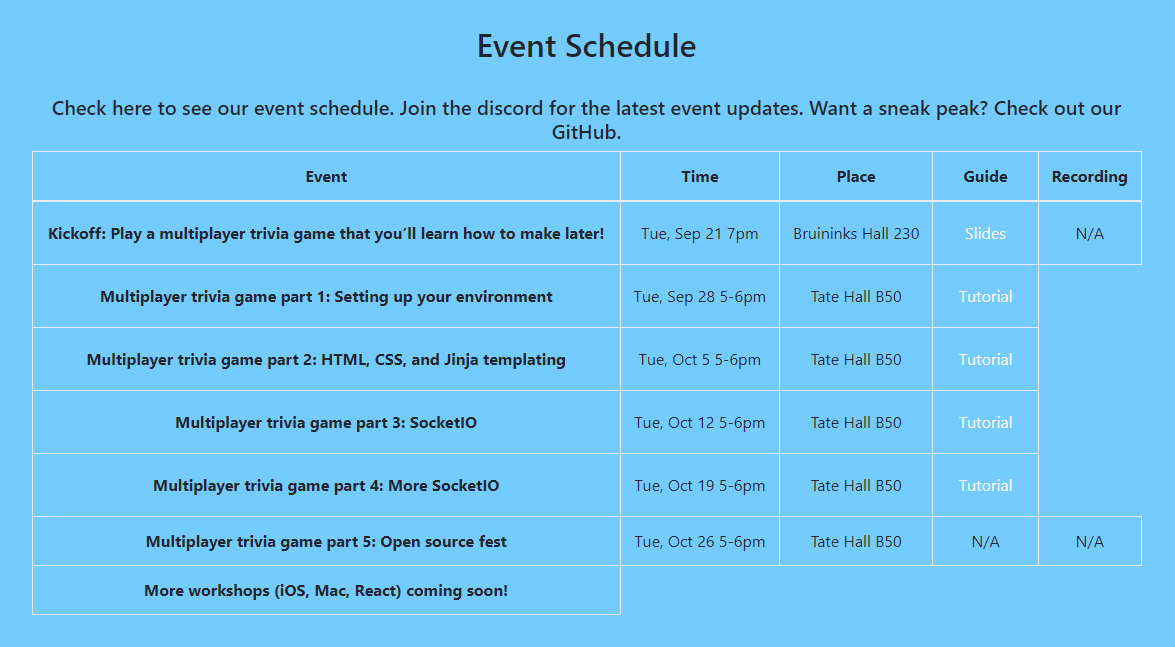
\includegraphics[width=0.9\textwidth]{schedule.png}
\end{frame}

\begin{frame}{Gauge the room}
	How many of these have you heard of? How many of these have you used?

	\begin{itemize}
		\item HTML
		\item CSS
		\item Flask
		\item JavaScript
		\item Socket-IO
	\end{itemize}
\end{frame}

\begin{frame}{Interest?}
	What do you want out of workshops? What do you want out of the club?

	\bigskip

	Would less structured events to simply meet collaborators for projects
	be helpful, or do you just want to meet on the discord?
\end{frame}

\begin{frame}{Follow the guide!}
	\centering
	\href{https://z.umn.edu/adc-mtg}{https://z.umn.edu/adc-mtg}

	\bigskip

	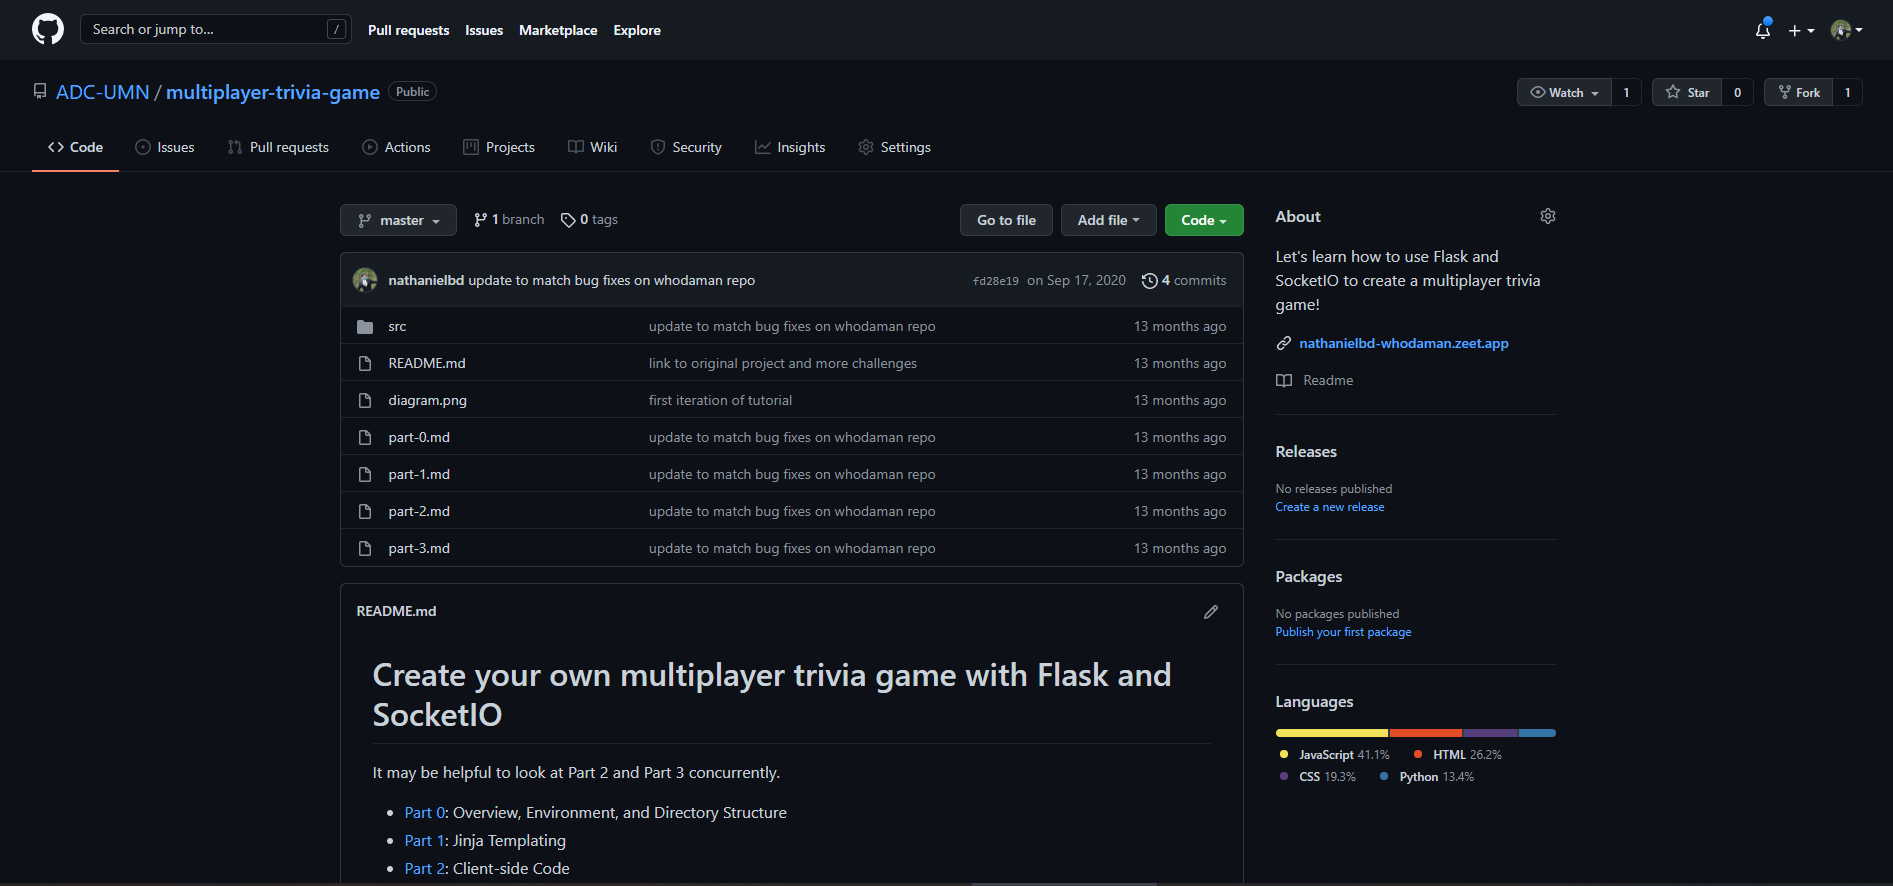
\includegraphics[width=0.9\textwidth]{guide.png}
\end{frame}

\begin{frame}{Python}
	Programming language, runs on a server

	\bigskip

	Let's install it: \href{https://www.tutorialdocs.com/tutorial/python3/setup-guide.html}{https://www.tutorialdocs.com/tutorial/python3/setup-guide.html}
\end{frame}

\begin{frame}{VS Code}
	\underline{Visual Studio} Code

	\bigskip

	Integrated Development Environment (IDE), text editor

	\bigskip

	\href{https://code.visualstudio.com/}{https://code.visualstudio.com/}
\end{frame}

\begin{frame}{The big picture}
	\centering
	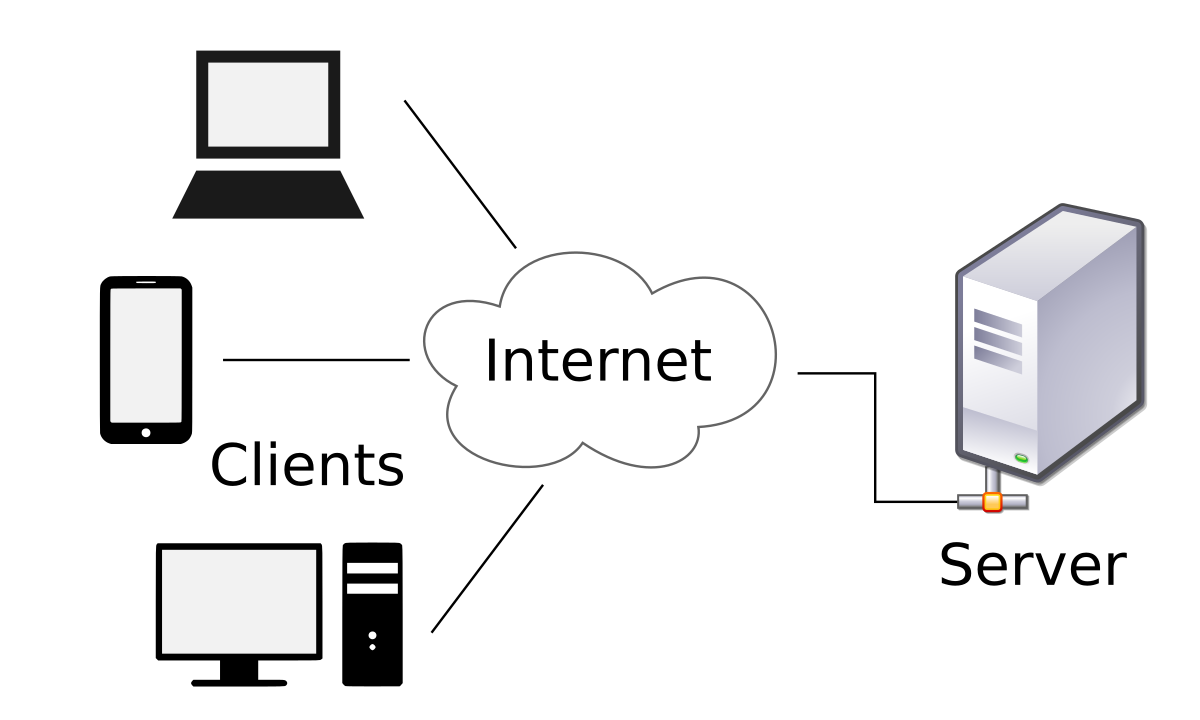
\includegraphics[width=0.9\textwidth]{client-server.png}
\end{frame}

\begin{frame}{Client side}
	\begin{columns}
		\begin{column}{0.5\textwidth}
			Client
			\begin{itemize}
				\item HTML
				\item CSS
				\item JavaScript
			\end{itemize}
		\end{column}
		\pause
		\begin{column}{0.5\textwidth}
			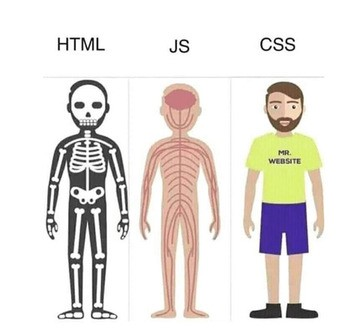
\includegraphics[width=0.9\textwidth]{web-tech.jpeg}
		\end{column}
	\end{columns}
\end{frame}

\begin{frame}{Server side}
	\only<1>{
		Server
		\begin{itemize}
			\item Flask
			\item Flask-SocketIO
		\end{itemize}	
	}
	\only<2>{
		\centering
		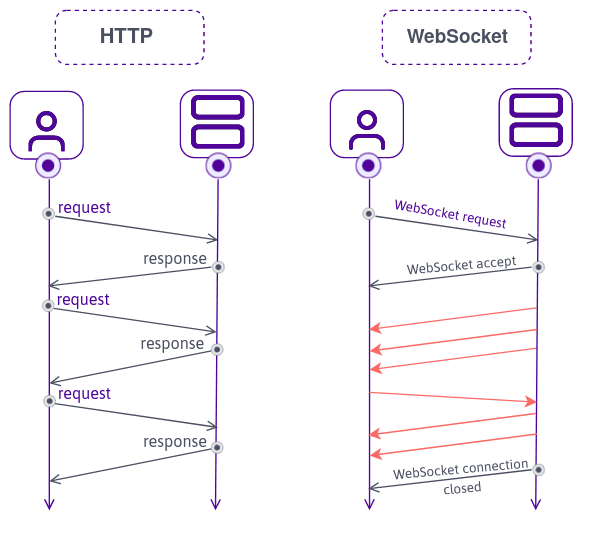
\includegraphics[width=0.7\textwidth]{ws.png}
	}
\end{frame}

\begin{frame}{What do I type?}
	\centering
	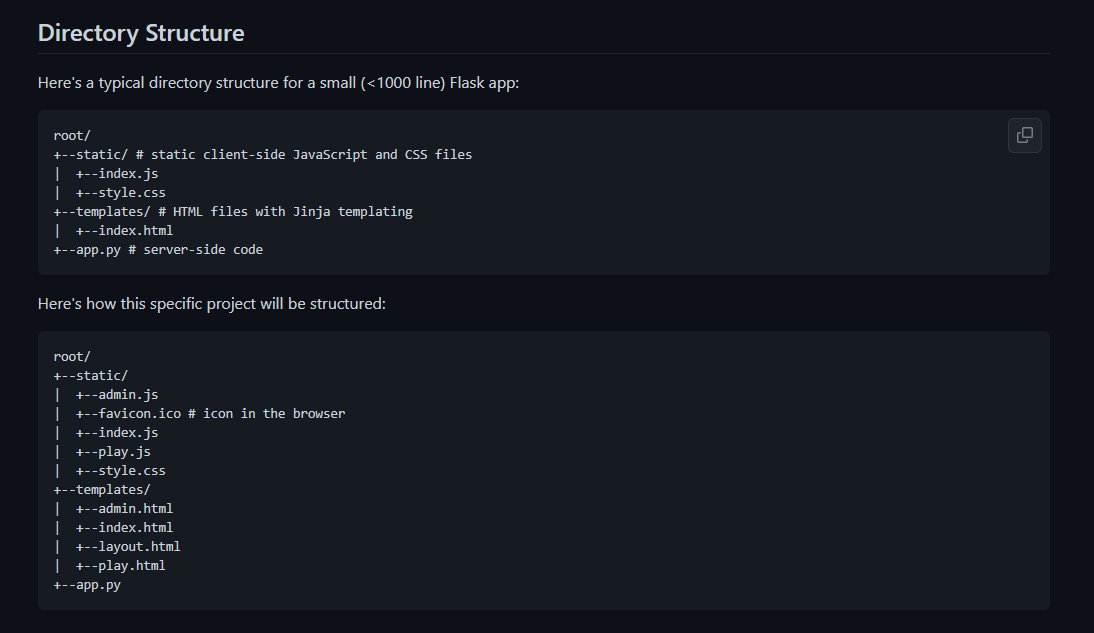
\includegraphics[width=0.9\textwidth]{directory.png}
\end{frame}

\begin{frame}{SocketIO events}
	\centering
	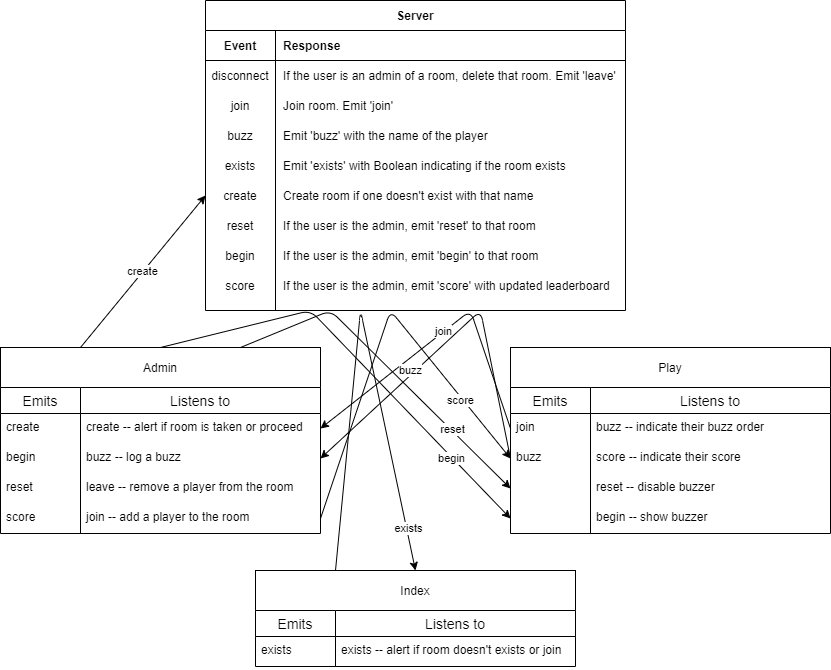
\includegraphics[width=0.8\textwidth]{../diagram.png}
\end{frame}

\end{document}